
\documentclass{article}
\usepackage{graphicx}
\usepackage{booktabs}
\usepackage{hyperref}
\usepackage{amsmath}
\usepackage{geometry}
\usepackage{cite}
\geometry{margin=1in}

\title{Why Naive Binary Representation Fails for LLM Efficiency}
\author{Sushanth Tiruvaipati}
\date{July 2025}

\begin{document}

\maketitle

\begin{abstract}
We investigate the impact of representing code in binary and assembly form when prompting large language models (LLMs). Contrary to the intuitive belief that machine code may be more efficient for models to process, our analysis across 60 code tasks and four prompt types reveals a staggering token inflation of over 14,000\% for binary representations. We show that naive binary encoding leads to massive cost overheads, making it a poor choice for efficient LLM inference.
\end{abstract}

\section{Introduction}
Token economy is critical in optimizing LLM workflows. With increasing interest in low-level code representation—such as hexadecimal binary and assembly—for compression or obfuscation, we explore the practical implications on token count and API cost. This paper presents empirical evidence that naive binary prompts are not only less efficient but also significantly more expensive than their source or assembly counterparts.

\section{Methodology}
We used a pipeline that compiled C code into binary and assembly formats and fed them into GPT-4 via prompts for four tasks: explanation, optimization, debugging, and conversion. For each prompt, we measured:
\begin{itemize}
  \item Token counts for source, binary, and assembly formats.
  \item Percentage savings (or inflation) in tokens.
  \item Estimated API costs assuming 500 output tokens per prompt.
\end{itemize}

\section{Results}

\subsection{Token Inflation}
\begin{itemize}
  \item \textbf{Binary representation}: 14,543\% token increase on average.
  \item \textbf{Assembly representation}: 903\% token increase on average.
  \item \textbf{Worst-case binary inflation}: 48,045\%.
\end{itemize}

\subsection{Cost Impact}
\begin{itemize}
  \item Total cost for source prompts: \$2.15.
  \item Cost for binary prompts: \$42.88 (1896\% increase).
  \item Assembly prompts cost: \$5.44 (153\% increase).
\end{itemize}

\begin{figure}[h!]
  \centering
  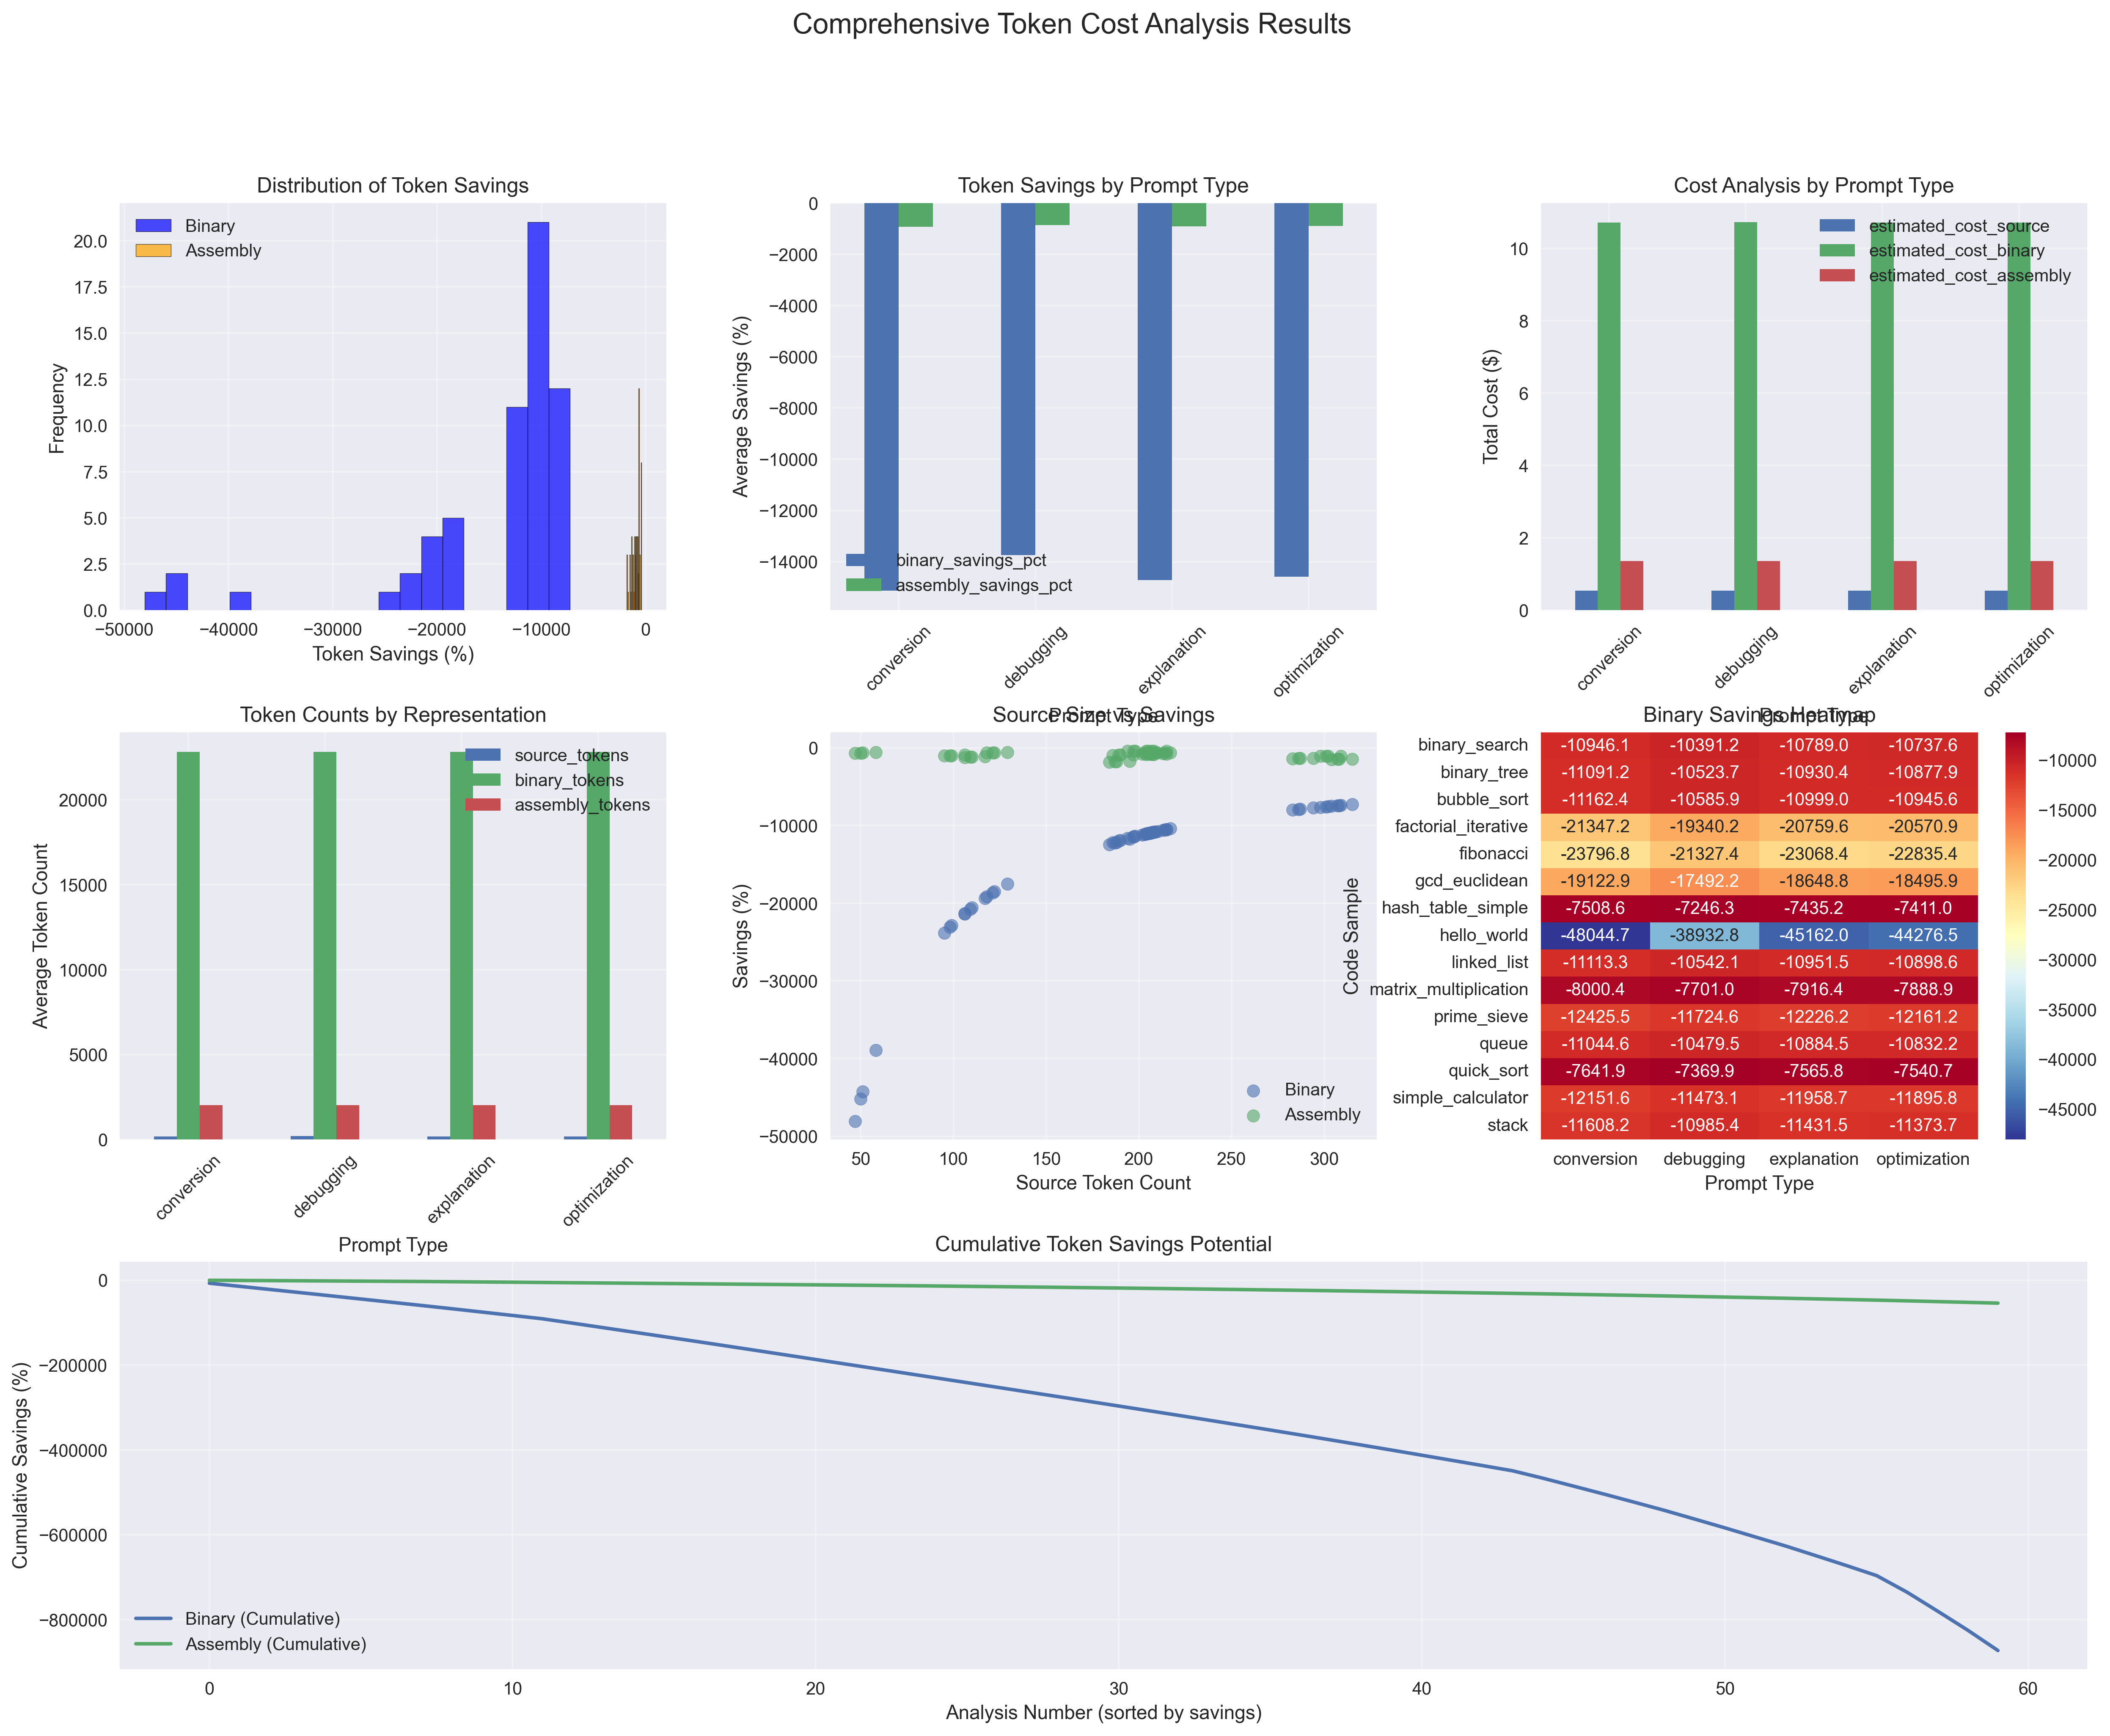
\includegraphics[width=\linewidth]{comprehensive_analysis_results.png}
  \caption{Visualization of token inflation and cost comparison across binary, assembly, and source code representations.}
\end{figure}

\section{Discussion}
The results clearly show that naive binary representation not only fails to reduce token count—it explodes it. This is due to the inefficiency of LLM tokenizers with hexadecimal strings and the loss of high-level structure in compiled formats. While binary may seem “smaller” on disk, it expands dramatically in tokenized form.
This finding complements our prior work on improving output diversity through model and temperature rotation \cite{uniqueness2025}.

Assembly offers a middle ground, being more readable and still somewhat more efficient than binary, though worse than source.

\section{Implications}
\begin{itemize}
  \item Binary prompts should be avoided in production LLM applications aiming for efficiency.
  \item Source and assembly formats remain superior for interpretability and cost.
  \item Cost savings alone do not justify low-level prompts—model accuracy must also be considered.
\end{itemize}

\section{Conclusion}
Naive binary prompts catastrophically increase token count and cost when interacting with LLMs. These findings advocate for caution when exploring token compression through binary encoding. Future research should examine model performance and accuracy with binary and assembly inputs before considering such representations viable.

\section*{Acknowledgements}
Thanks to the open-source and AI research communities for tools that made this analysis possible.

\begin{thebibliography}{9}

\bibitem{uniqueness2025}
S. Tiruvaipati,
\textit{Enhancing Output Uniqueness in Large Language Models via Model Rotation, Temperature Tuning, and Embedding-Based Validation}, 
ResearchGate Preprint, 2025.
Available: \url{https://www.researchgate.net/publication/393715387_Enhancing_Output_Uniqueness_in_Large_Language_Models_via_Model_Rotation_Temperature_Tuning_and_Embedding-Based_Validation}

\end{thebibliography}

\end{document}
